\subsection{Performance Evaluation}

While \sysname\ can effectively eliminate redundant files in the
Docker registry, it introduces overheads which can reduce the
registry's performance.
%
%The overheads can be classified in two categories: 1)~\emph{background
%overhead} caused by the computation and I/O that is performed during layer
%deduplication; and 2)~\emph{foreground overhead} from extra processing on the
%critical path of a pull request.

\begin{figure}
	\centering
	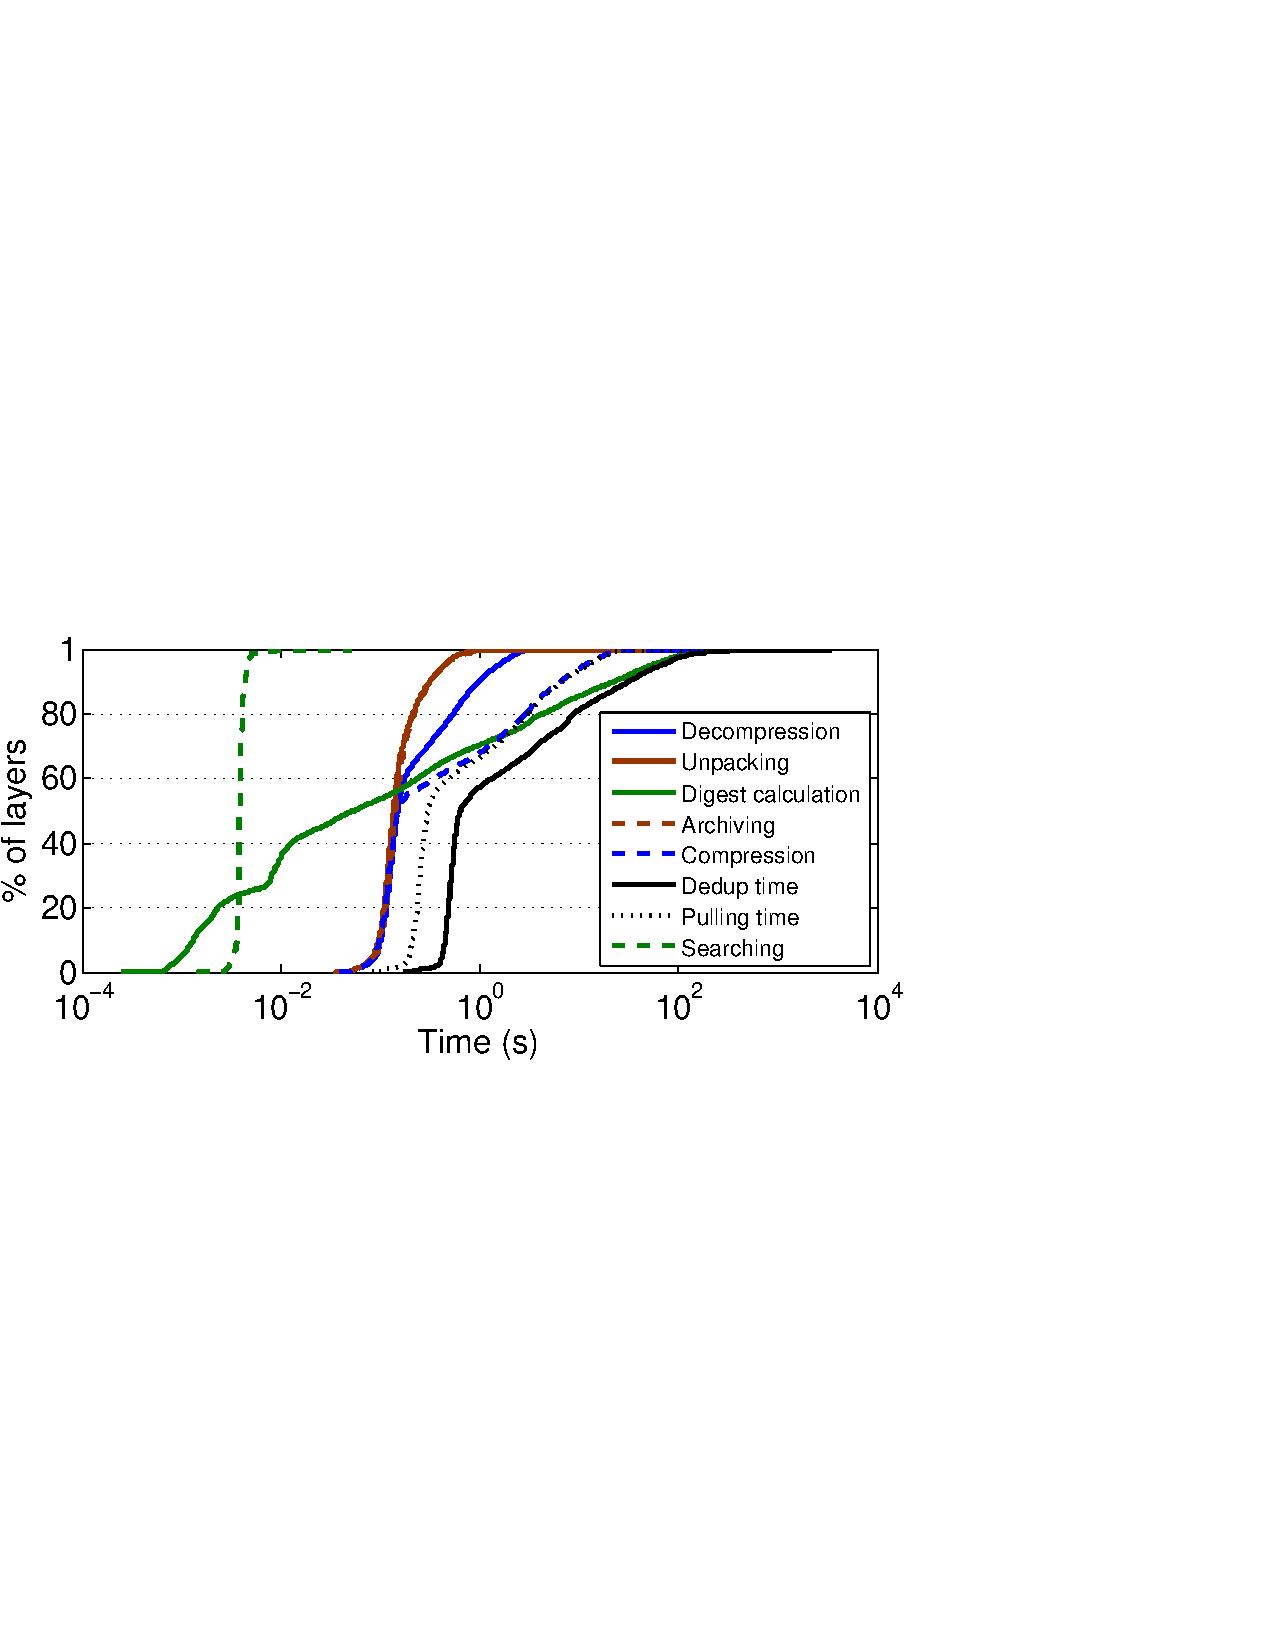
\includegraphics[width=0.5\textwidth]{graphs/res-time.pdf}
	\caption{Off-line file-level deduplication run time.}
	\label{fig:dedup-res}
\end{figure}


\paragraph{Simulation}
%
To analyze the impact of file-level deduplication on performance,
we conducted a preliminary simulation of \sysname.
%
%Based on the simulation results, we estimated the overhead of \sysname\ on
%\texttt{push} and \texttt{pull} layer request latencies.
%
%We then provide different suggestions on how the Docker registry can mitigate
%the deduplication overhead.
%
%%%%%%%%%%%%%%%%%%%%%%%%%%%%%%%%%%%%%%%%%%%%%%%%%%%%%%%%%%%%%%%%%%%%%%%%%%%%
%
%
Our simulation
approximates several \sysname's steps described in Section~\ref{sec:design}.
%
First, a layer from our dataset is copied to a RAM disk. 
%
%
%Note that there is no foreground pull or push requests since the simulation is \emph{off-line}.
%
The layer is then decompressed, unpacked, and the fingerprints of all files
are computed using the MD5 hash function~\cite{MD5}.
%
The simulation searches the fingerprint index for duplicates,
and, if the file has not been stored previously, it records the
file's fingerprint in the index.
%
%To map a layer to its containing files, we create the layer recipe and add it
%to a \emph{layer-to-file table}.
%
%The simulator then creates a file recipe.
%
%For each file in a layer, a layer digest
%to its containing file content digest mapping record is also created 
%
%The \emph{layer-to-file table} also
%records the file path within each layer associated with each file.
%
Note that at this point our simulation does not include
the latency of storing unique files.
%
To simulate layer's reconstruction during the \texttt{pull},
we archive and compress corresponding files.
%
%Only unique files are maintained in RAM
%disk while the redundant copies are removed.
%

We implemented the simulation in 600 lines of Python code
and setup a one-node Docker registry on a machine with 32~cores and 64GB of RAM.
%
To speed up the experiments and fit the required data in the RAM
we used 50\% of all layers and excluded the ones larger than 50MB.
%
We processed 60 layers in parallel using 60 threads.
%
The overall runtime of the simulation was roughly 3.5 days.
%
%The overall runtime is about 3.5 days.

Figure~\ref{fig:dedup-res} shows the CDF for each sub-operation of
\sysname.
%
Unpacking, Decompression, Digest Calculation, and Searching 
are part of
the deduplication process and together make up the Dedup time.
%
\VT{@Nannan, in Figure ~\ref{fig:dedup-res} can you reorder the lines in the
legend so that the Searching goes after Digest calculation?}
%
Searching, Archiving, and Compression
simulate the additional processing for a \texttt{pull}
request and form the Pulling time.
%

%\LR{What was the overall runtime for processing 0.9 million layers?}\NZ{addressed}
%
%\alicomment{How are we saving the location
%of each file in the layer? It is not clear from the following sentences.}
%\NZ{addressed}
%
%To improve searching performance, the
%mapping table is stored in Hive database~\cite{xxx}. 
%
%\lrcomment{Why are we using Hive for this? It seems overkill to me, especially
%for such small data. Even at scale, a KeyValue store would probably provide
%better performance than clunky MapReduce-based DB.}
%

\paragraph{Push}

\sysname\ does not directly impact the latency of \texttt{push} requests because
deduplication is performed asynchronously, \ie the registry reliably stores a
copy of the layer as-is and then sends a response to the client.
%
The appropriate performance metric for push is the time it takes to deduplicate
a single layer.
%
%Next, we look at the effects on \texttt{push} and \texttt{pull} latencies in
%more detail.
%
%However, if there are intensive push requests while the registry is performing
%deduplication, \sysname\ can still impact push latencies because it incurs
%CPU, memory, and I/O overhead. %(similar to pull requests).
%
Looking at the breakdown of the deduplication time in
Figure~\ref{fig:dedup-res}, we make several observations.
%
First, the searching time is the smallest among all operations with 90\% of the
searches completing in less than 4ms and the median of \VT{XXX}ms.
%
%The mapping table maintains 0.98 million layer-to-file digest mapping records. 
%
%\LR{Remove the following sentence? 1.7 million records is actually quite small
%so even a single-node DB with one index is enough.}\NZ{addressed} Consider
%that more than 1.7 million layers are stored in Docker hub and the number is
%still increasing, it's better to choose a fast distributed database to provide
%high searching performance and scalability.
%
Second, the calculation of digests spans a wide range from 5$\mu$s to almost
125s.
%
%This is because the time mainly depends on the layer size, \ie the fewer and
%smaller files a layer contains, the faster it is to compute all digests for
%the layer.
%
%Typically, smaller layers contain a smaller number of smaller files, which
%takes much less time to calculate their digests.
%
%While if the layer is bigger, the digest calculation overhead will be higher. 
%
90\% of digest calculation times are less than 27s while 50\% are
less than \VT{XXX}s.
%
The diversity in the timing is caused by a high variety of layer sizes both in
terms of storage space and file counts.
%
%Thus, we suggest that multiple-threading is needed to calculate the files'
%digests simultaneously; 
%
%Fast CPUs as well as more powerful computing nodes are required to speed up
%digest calculation.
%
Third, the run time for decompression and unpacking follows identical
distribution for approximately 60\% of the layers and is less than 150ms.
%
%Around 60\% of decompression and unpacking time are less than 0.15\,s. 
%
However, after that, the times diverge and compression times increase faster
compared to unpacking times.
%
\VT{do we have some theory why?}
%
90\% of decompressions take less than 950ms while 90\% of packing time is less
than 350ms.

%Overall, we see that file digest calculation contributes a lot to the
%overall deduplication latency especially when the layer size is big.  Moreover,
%we see that the deduplication latency increases as the layer size grows.
%
Overall, we see that 90\% of file-level deduplication time is less than \VT{XXX}s
per layer, while the average processing time for a single layer is \VT{XXX}.
%
This means that our single-node deployment can process about 3 layers/s on average.
%
In future we will work on further improving \sysname's deduplication throughput.
%
%In a large-scale registry deployment, this throughput can be improved
%as more node are available to perform deduplication.
%

\paragraph{Pull} 

From Figure~\ref{fig:dedup-res}
we can see that around 55\% of the layers have close compression and archiving
times ranging from from 40ms to 150ms and both operations contribute equally
to pulling latency.
%
%60\% of compression and archiving time are less than 0.15 s.
%
%While compression has the highest run time 80\% of compression time is less than 2.82~s. 
%
%\LR{Again, better to show the 90th percentile.}
%\NZ{90\% of the compression time is less than 8\,s.}
After that, the times diverge and compression times increase faster with an
90\textsuperscript{th} percentile of 8s.
%
This is because compression times increase for larger layers and follow the distribution
of layer sizes (see Figure~\ref{fig:layer-size-cdf}).
%
%80\textsuperscript{th} percentile of 2.82\,s.
%
Compression time makes up the major portion of the pull latency and becomes a
bottleneck.
%
%We see that archiving time and compression contributes equally to pulling
%latency when their run time are lower than 0.15 s while compression time almost
%equals to pulling latency when the compression time is greater than 0.15 s. 
